\section{ \SpecLang Specifications}
\label{sect:spec}

We  now discuss   syntax and semantics of \SpecLang specifications, and illustrate through examples.

\subsection{\SpecLang syntax }

Our specifications language, \SpecLang,  supports the one state invariants, two state invariants,  method specifications, and the conjunction of such specifications:
 
\begin{definition} [\SpecLang Specifications]   We define the \emph{syntax} of \SpecLang:
\noindent

\label{f:holistic-syntax}
\[
\begin{syntax}
\syntaxElement{S}{}
		  {\syntaxline
                                 {\OneStateQ {\overline {x:C}} {A} }	
				{\TwoStatesQ {\overline {x:C}} {A} {A} }	
				{ \sdN{\mprepost{A}{C}{m}{x}{C}{A} }} %{A[\!\![ \,C\!::\!m(\overline{x:C})\,]\!\!] A }}
				{S\, \wedge \, S}
		 \endsyntaxline
		}
\endSyntaxElement\\
\end{syntax}
\]
\sdN{Specifications'    \emph{well-formedness},  $\vdash S$,  is   defined by cases on $S$: \ \  \
 $\vdash {\OneStateQ {\overline {x:C}} {A}}$  if  $fv(A)\subseteq\{  \overline x \}$;\ \ \   \ \ 
 $\vdash {\TwoStatesQ {\overline {x:C}} {A} {A'}}$  if    $fv(A), fv(A')\subseteq \{ \overline x \}$; \ \ \ \  \
 $\vdash {\mprepost{A}{C}{m}{x}{C}{A} }$   if      $fv(A')\subseteq  fv(A)\cup \{\prg{res}, \prg{this}, \overline x\}$; \ \   \ \ \
 $\vdash S\, \wedge \, S'$  if  $\vdash S$   and   $\vdash S'$.  
}
\end{definition}

We now consider some examples.

 \sdN{\begin{example}[One-state Invariants]
 \label{example:oneState}
  $S_{10}$  guarantees   that  the balance is never negative:
  \\
   \begin{tabular}{lcll}
$\strut \ \ \ \ \ \ \ \ S_{10}$ & $\triangleq$   & ${\OneStateQ {\prg{a}:\prg{Account}} {\prg{a.balance} \geq 0}}$
 \end{tabular}
  
 \end{example}
}

\sdN{
 \begin{example}[Two-state Invariants]
 \label{example:twostate}
  % 
 $S_5$  guarantees   that   non-null passwords do not change:
 \\
 \begin{tabular}{lcll}
%$S_{2a}$   &     $\triangleq$   &   ${\TwoStatesQ {\prg{a}:\prg{Account}.\prg{p}:\prg{Password}}  {\prg{p}=\prg{a.password} \wedge \inside{\prg{p}}}{\inside{\prg{p}}} }$
% \\
$\strut \ \ \ \ \ \ \ \ S_5$ & $\triangleq$   & ${\TwoStatesQ {\prg{a}:\prg{Account}.\prg{p}:\prg{Password}}  {\prg{null}\neq \prg{p}=\prg{a.password}} {\prg{p}=\prg{a.password}} }$
 \end{tabular}
 \end{example} 
 }
 
\sdN{ \begin{example}[Method Specifications]
 \label{example:mprepostl}
Here we have two specifications for \prg{transfer}:\ $S_6$   guarantees that
accounts different than from the receiver and argument are not affected, and that if the password supplied is not that of the receiver, then no account's balance if affected.
$S_7$ guarantees that if the password supplied is that of the receiver, the correct amount is transferred from the receiver to the destination.
 $S_8$ guarantees that \prg{set} preserves the protectedness of a password.
% The specifications from below describe properties ot the methods \prg{set}  and \prg{transfer}:
\\
{\sprepost
		{\strut \ \ \ \ \ \ \ \ \ S_6} 
		{ a:\prg{Account}\wedge 
		(\prg{dst}\neq a\neq\prg{this} \vee \prg{pwd'}\neq\prg{a.passwd} \wedge a.\prg{balance}=b}
	               {\prg{Account}} {\prg{transfer}} {\prg{dst}:\prg{Account},\prg{pwd'}:\prg{Password},\prg{amt}:\prg{int}}
		{ a.\prg{balance}=b}
}
\\
{\sprepost
		{\strut \ \ \ \ \ \ \ \ \ S_7} 
		{ % b,b':\prg{int} \wedge  
		\prg{this}\neq \prg{dst}\wedge \prg{this}.\prg{balance}=b \wedge  \prg{dst}.\prg{balance}=b' }
		  {\prg{Account}} {\prg{transfer}} {\prg{dst}:\prg{Account},\prg{pwd'}:\prg{Password},\prg{amt}:\prg{int}}
		{\prg{this}.\prg{balance}=b-\prg{amt} \wedge \prg{dst}.\prg{balance}=b'+\prg{amt}}
}
\\
{\sprepost
		{\strut \ \ \ \ \ \ \ \ \ S_8} 
		{ %a:\prg{Account}\wedge
		 \inside{a.\prg{password}}}
		{\prg{Account}} {\prg{set}} {\prg{pwd'}:\prg{Password}}
		{ \inside{a.\prg{password}}}
}
\\
{\sprepost
		{\strut \ \ \ \ \ \ \ \ \ S_9} 
		{ %a:\prg{Account}\wedge
		 \protectedFrom{\prg{this}.\prg{myAccount}.\prg{pwd}} {buyer} \wedge \prg{this}.\prg{myAccount}.\prg{balance}=b
		 }
		{\prg{Shop}} {\prg{buy}} {\prg{buyer}:\prg{external}, \prg{anItem}:\prg{Item} }
		{ 
		  \protectedFrom{\prg{this}.\prg{myAccount}.\prg{pwd}} {buyer} \wedge \prg{this}.\prg{myAccount}.\prg{balance}\geq b
		 }
}
%\\
%{\sprepost
%		{\strut \ \ \ \ \ \ \ \ \ S_{9}}
%		 {% a:\prg{Account}\wedge 
%		 a.\prg{password}\neq \prg{pwd'} \wedge a.\prg{balance}=b}
%				       {\prg{Account}} {\prg{transfer}} {\prg{dst}:\prg{Account},\prg{pwd'}:\prg{Password},\prg{amt}:\prg{int}}
%		{ a.\prg{balance}\geq b}
%}
%resp that the balance of any account ...TODO ... explain ...
\end{example}
}

\subsection{\SpecLang  Semantics}
%\subsubsection*{Arising States} % and {Arising} External States}
\footnoteSD{TODO motivate;
Here what we had: As discussed in \S \ref{s:approach}, 
{open world specifications need to be able to provide}
guarantees which hold
during execution of an internal, 
known, trusted module $M$ when linked together with any
unknown, untrusted, module $M_{ext}$. These guarantees need only hold 
when the external module is executing; we are not concerned if they are
temporarily broken by the internal module. Therefore, we are only interested in states where the
executing object (\prg{this}) is an external object. 
To express our focus on external states, we define the  \emph{external states semantics}, of the form 
$\reduction{M_{ext}}{M}{\sigma}{\sigma'}$, where $M_{ext}$ is the external
module, and $M$ is the internal module, and where we
collapse all internal steps into one single step.
}
{{Our specifications  describe  properties of states which \emph{arise} from the execution of our module combined with other, external modules, and
%The first state must be a state that may \emph{arise} from the execution of the module, defined below. 
%We require that execution 
starting at an \emph{intitial} state. %A state $\sigma$ is \emph{arising},}  written $\arising{\sigma}{M}$, {if it  may arise}  % by observable states} 
%by execution
% starting at some initial configuration:


\begin{definition}[Arising  States]
\label{def:arising}
For modules $\overline M$ we define arising  states as follows:

\begin{itemize}
\item
 a state $\sigma$ is 
{ an \emph{arising} state, formally \ \ \  $\arising{\sigma}{\Mtwo}$,\ \ \ if  there exists some $\sigma_0$ such that $\initial{\sigma_0}$ and
$\Mtwo, {\sigma_0} \leadstoN^* {\sigma}$.}
%\item
%{A a state $\sigma$ is 
%called an \emph{arising} state, formally\ \ \ \  $\extArising{\sigma}{M_{ext}}{M}$,\ \ \ \
%if and only if $\arising{\sigma}{M_{ext}*M}$ and $M, \sigma \models \external{\prg{this}}$.}
\end{itemize}
\end{definition}
  
We now move to the semantics of \SpecLang Specifications, and   define what it means for  a module  $M$ to satisfy specification  $S$, written as $M \vDash S$.  
 
\begin{definition}% [Semantics of \SpecLang Specifications]

We define $\satisfies{M}{{S}}$ by cases over the four possible syntactic forms.

\label{def:necessity-semantics}

\begin{enumerate}
\item
$
\satisfies{M}{ \OneStateQ {\overline {x:C}} {A} } \  \ \ \ \ \ \ \ \ \ \ \ \ \ \mbox{iff}  \     
    \begin{cases}
     \mbox{for all }   \Mtwo  \mbox{ and }  \sigma:\\
   \ \ \ \  [\ \ \   \arising{\sigma}{M\madd\Mtwo}  \ \  \wedge\ \ M, \sigma  \models {\external{\prg{this}}} \\
    \ \ \ \ \ \   \ \ \ \Longrightarrow\\
    \ \ \ \ \ \  \  \satisfiesA{M}{\sigma}{\forall \overline{x:C}.A}\ \  \  ] 
    \end{cases} 
 $
 \item
 $\satisfies{M}{\TwoStatesQ {\overline {x:C}} {A}{A'}}   \ \, \ \ \ \ \mbox{iff}  \   \
    \begin{cases}
     \mbox{for all }   \Mtwo,  \sigma, , \sigma', \mbox{ and }  \overline{\alpha}    \\
 \ \ \ \  [ \ \ { \arising{\sigma}{M\madd \Mtwo }\   \  \wedge\ \ \GRelevant {\overline \alpha}  \sigma}\ \ \ \wedge  \\
  \ \ \ \  \ \ \  \satisfiesA {M}   {\sigma}  {(\overline {\alpha :C} \ \wedge\  {A[\overline{\alpha/x}]}\ \wedge \  {\external{\prg{this}}}) } \ \ \ \wedge   \\
 \ \ \ \   \ \ \ {\leadstoBoundedStar {M\madd \Mtwo}{\sigma}  {\sigma'} } \ \ \wedge\ \  M, \sigma' \models {\external{\prg{this}}}  \\
 \ \ \ \   \ \ \ \ \  \ \Longrightarrow   \\
 \ \ \ \   \ \ \  {\satisfiesA{M}{\sigma'}{ A'[\overline{\alpha/x}]}  }  \ \ \  ]  
     \end{cases} 
 $
 \item
\red{ $\satisfies{M}{\mprepost{A}{C}{m}{x}{C}{A'} }   \ \,  \mbox{iff}  \   \ 
    \begin{cases}
     \mbox{for all }   \Mtwo,  \sigma, \sigma'  \mbox{ and variables}\, z, y,\overline{y}    \\
   \ \ \ \  [ \ \ { \arising{\sigma}{M\madd \Mtwo} }\    \ \ \wedge \ \  \sigma.\prg{cont}\txteq z=y.m(\overline y)
 \ \ \ \wedge  \\
 \ \ \ \   \ \ \    \satisfiesA {M}   {\sigma}  {(y: C \, \wedge \, \overline {y :C} \, \wedge  \, {A[ y/\prg{this},  \overline{y/x} ] }\,) }  \ \ \wedge\\  
 \ \ \   \ \ \  \ {\leadstoBoundedStarFin {M\madd \Mtwo}{\sigma}  {\sigma'} }     \\
 \ \ \ \   \ \ \ \ \  \ \Longrightarrow   \\
 \ \ \ \   \ \ \  {\satisfiesA{M}{\sigma'}{ A'[ {z/\prg{res},  y/\prg{this},  \overline{y/x}] } } } \  \ ]
    \end{cases} 
    $
 }
 \item
 $\satisfies{M}{S\, \wedge\, S'}$ \ \ \ \ \ \ \ \ \ \ \ \ \ \ \ \ \ \ \  \ \ \  iff  \  \ \  \   $\satisfies{M}{S}\ \wedge \ \satisfies{M}{S'}$
\end{enumerate}


%\begin{tabular}{l l c l }
%
%$(1)$ & $\satisfiesA{M}{ \OneStateQ {\overline {x:C}} {A} }$ & iff & 
%for all $\Mtwo$, and $\sigma$  \\
%  & & & $[ \ \  \arising{\sigma}{M\madd\Mtwo}  \ \  \wedge\ \ M, \sigma  \models {\external{\prg{this}}} % \ \wedge 
%$\\
%& & & $\ \ \ \ \  \ \Longrightarrow \  $ \\ % \\ & & &  $ \satisfiesA{M}{\sigma[\overline{x\mapsto o}]}{A} $
%& & & \ \ \   {$ \satisfiesA{M}{\sigma}{\forall \overline{x:C}.A}\ \ ] $}
%\\
%\\
%$(2)$ & $\satisfies{M}{\TwoStatesQ {\overline {x:C}} {A}{A'}}$& iff & 
%for all $\Mtwo$, $\sigma$,   and $\overline{\alpha}$   \\
% & & & $[ \ \ { \arising{\sigma}{M\madd \Mtwo }\   \  \wedge\ \ \GRelevant {\overline \alpha}  \sigma}\ \ \ \wedge$ \\
% & & & $\ \ \  \satisfiesA {M}   {\sigma} {\red{(\overline {\alpha :C}}\ \wedge\  \red{A[\overline{\alpha/x}]}\ \wedge \  {\external{\prg{this}}}) } \ \ \ \wedge $ \\
% % \ \ \wedge \satisfiesA{M}  \sigma   {\external{\prg{this}}} \ \ \wedge $ \\
% %\ \    \satisfiesA{M}   {\sigma[\overline{x\mapsto \alpha}]}{(\overline {x:C} \wedge A)} \ \ \ \wedge}$ \\ 
% & & & $\ \ \ {\leadstoBoundedStar {M\madd \Mtwo}{\sigma}  {\sigma'} } \ \ \wedge\ \  M, \sigma' \models {\external{\prg{this}}}$ \\
%& & & $\ \ \ \ \  \ \Longrightarrow $ \\
%& & & $\ \ \  \satisfiesA{M}{\sigma'}{\red{A'[\overline{\alpha/x}]}} \ \ ] $
%\\
%\\
%$\bullet$ &  $\satisfies{M}{S\, \wedge\, S'}$ &   iff   & $\satisfies{M}{S}\ \wedge \ \satisfies{M}{S'}$
%\end{tabular} 

 
\end{definition} 


\footnoteSD{First bullet: This means that we require all objects to satisfy even if not locally relevant. Second Bullet: notice that we are asking for globally relevant objects}  
\footnoteSD{{TODO: Make an example that demonstrates the difference if in the second bullet we had asked for locally relevant objects ${\overline o}$.}}
\footnoteSD{{TODO Notice that we assume that $\overline x$ are not free in $A$ -- cf Barendregt convention.}}
\footnoteSD{TODO: explain why we did not require the stronger $\leadstoFin{M_{ext}\!\circ \!M}{\sigma}{\sigma'}$ rather than $\leadstoBoundedStar {M_{ext}\!\circ \!M}{\sigma}  {\sigma'}$.}
% Note that the requirements that $\extArising{\sigma}{M_{ext}}{M}$ and $\leadstoFin{M_{ext}\circ M}{\sigma}{\sigma'} $ imply that
% $M, \sigma' \models {\external{\prg{this}}}$



We demonstrate the meaning of ${\TwoStatesQ {\overline {x:C}} {A_0}{A_0}}$ in Fig. \ref{fig:illusrPreserve} where we refine the execution shown in Fig. \ref{fig:UpSemantics}, and take it that the pink states, \ie   ${\sigma_6}$-${\sigma_9}$ and $\sigma_{13}$-$\sigma_{17}$, and  $\sigma_{20}$, $\sigma_{21}$ are external, and the green states, \ie   ${\sigma_{10}}$,  ${\sigma_{11}}$,   ${\sigma_{12}}$,  ${\sigma_{18}}$, and  ${\sigma_{19}}$, are internal. 
 
 \begin{figure}[htb]
\begin{tabular}{|c|}
\hline  % \\
\resizebox{8cm}{!}{
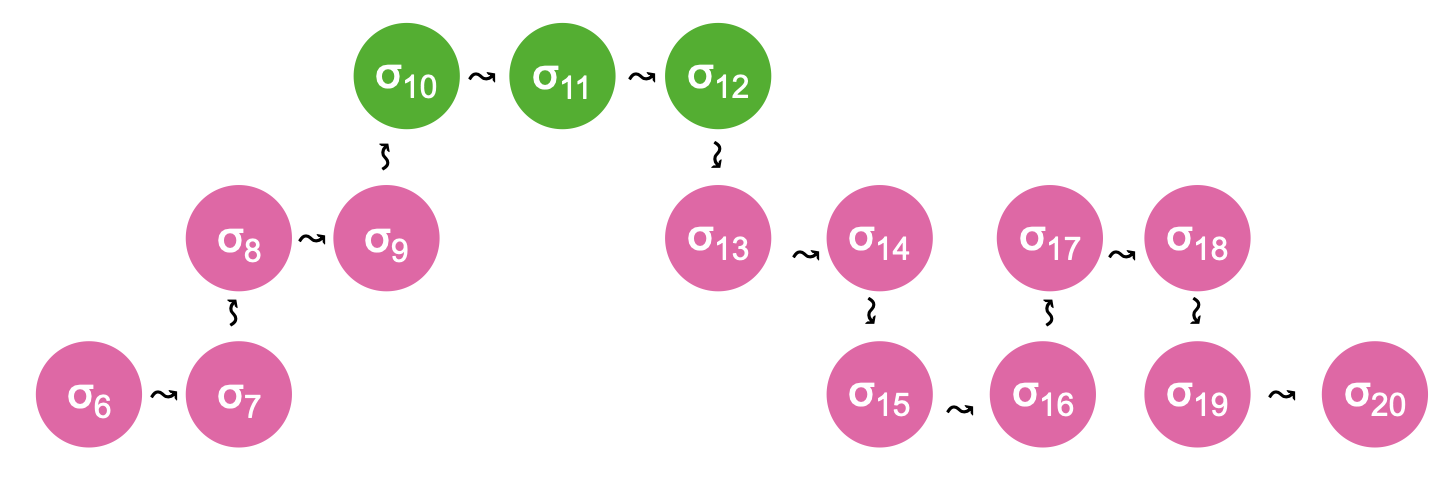
\includegraphics[width=\linewidth]{diagrams/preserves.png}, 
} 
\\
\hline
% \\
\begin{tabular}{lcl}
$\leadstoBoundedStar {...} {\sigma_6}   {\sigma_9} $ & & thus, $A_0$ guaranteed to be preserved from $\sigma_6$ to $\sigma_9$.\\
$\leadstoBoundedStar {...} {\sigma_6}   {\sigma_{13}} $ & & thus, $A_0$ guaranteed to be preserved from $\sigma_6$ to $\sigma_{13}$.\\
$\leadstoBoundedStar {...} {\sigma_6}   {\sigma_{19}} $, \ \  but $..,\sigma_{19}\not \models {\external{\prg{this}}}$ & & thus, $A_0$ not guaranteed to be preserved from $\sigma_6$ to $\sigma_{19}$.\\
$\leadstoBoundedStar {...} {\sigma_6}  {\sigma_{20}} $  \ \   & & thus, $A_0$  guaranteed to be preserved from $\sigma_6$ to $\sigma_{20}$.\\
$\notLeadstoBoundedStar {...} {\sigma_8}  {\sigma_{20}} $  \ \   & & thus, $A_0$  not guaranteed to be preserved from $\sigma_8$ to $\sigma_{20}$.\\
%$ {\sigma_6} \leadsto^*  \sigma_9 $ preserves $A_0$ & &
%$ {\sigma_6} \leadsto^*  \sigma_{10} $ does not preserve $A_0$ \\
%$ {\sigma_8} \leadsto^*  \sigma_{14} $ preserves $A_0$ & &
%$ {\sigma_8} \leadsto^* \sigma_{17} $ does not preserve $A_0$\\
%$ {\sigma_7} \leadsto^*  \sigma_{16} $  preserve $A_0$ & &
%$ {\sigma_9} \leadsto^*  \sigma_{19} $ does not preserve $A_0$
%\\
\hline
\end{tabular}
\end{tabular}
   \caption{Illustrating  the meaning on ${\TwoStatesQ {\overline {x:C}} {A_0}{A_0}}$  -- refining Fig. \ref{fig:UpSemantics}.  }
   \label{fig:illusrPreserve} 
 \end{figure}
 
% \subsection{\SpecLang Examples}
%\noindent
 \begin{example}
 \label{example:twostatesarisfy}
 \sdN{We now revisit the specifications given in Sect. \ref{s:bankSpecEx}, and the one from Example \ref{example:twostate}, and  the three  modules from Sect. \ref{s:bank}:}


\begin{tabular}{lllllllll}
$\ModA  \models S_1$  &   $\ModA  \models S_2$ &  $\ModA \models S_3$ &   $\ModA \models S_4$    & $\ModA \models S_5$\\
 $\ModB \models S_1$  &   $\ModB \not\models S_2$   &  $\ModB  \models S_3$   &  $\ModB  \not\models S_4$   & $\ModB \not\models S_5$ \\
 $\ModC  \models S_1$    & $\ModC \models S_2$ &   $\ModC \models S_3$    &$\ModC \not\models S_4$   & $\ModC \not\models S_5$ 
\end{tabular}
\end{example}
 

 \sdN{
 \begin{example}
 \label{example:mprepostlsatissy}
 Consider  the %method
  specifications   from Example \ref{example:mprepostl}.
Here, $\ModA \models S_6$ and $\ModB \models S_6$ and  $\ModC \models S_6$.
Also,  $\ModA \models S_7$ and $\ModB \models S_7$ and  $\ModC \models S_7$.
However,   $\ModA  \models S_8$, while $\ModB  \not\models S_8$.

Moreover,  for any method specification  $S \triangleq {\mprepost{A}{C}{m}{x}{C}{A'} }$ and any module   which does not have a class $C$  with a method $m$ with formal parameters types ${\overline C}$, we have that $M \models S$.
Namely, if a method were to be called with that signature on a $C$  from $M$, then execution would be stuck, and the requirements from Def. \ref{def:necessity-semantics}(3) would be trivially satisfied.
Thus,   $\ModC \models S_8$. %, even though $\ModC$ does not have a method \prg{set} with the signature given in $S_6$;

\end{example}
}
 
 
\subsection{\SpecLang Entailments}

\sdN{We define entailment of specifications wrt a module in the expected way.} %The usual definition of entailment applies to our specifications as well}

\begin{definition}[Satisfaction of Assertions by a module] 
\label{def:assertion-inference-semantics}
We define satisfaction of an assertion $A$ by a  module $M$ as:
\begin{itemize}
\item
{
$M \models A$   \ \ \ iff \ \ \  $\forall \overline{M}. \forall \sigma
[\ \    \arising{\sigma}{M\madd\overline{M}}\   \  \wedge\ \  \satisfiesA {M}   {\sigma} {\external{\prg{this}}} 
\   \ \Longrightarrow \ \ \satisfiesA{M}{\sigma}{A}\ \ ]$
}\footnote{Not sure about the need for external and arising.}
\end{itemize}
\end{definition}

%TODO: Here we will say that assertions are classical, as proven in FASE

\begin{definition}[Stronger Specifications] 
\label{def:specification-implication-semantics}
Specification $S$ is stronger than another specification $S'$  in the context of a  module: 
 \begin{itemize}[itemsep=5pt]
\item 
$\stronger M  S  {S'}$   \ \ \ iff \ \ \  $M\models S$ implies $M \models S'$
\item
$\strongerEq M  S  {S'}$   \ \ \ iff \ \ \ $\stronger M  S  {S'}$  \ and \  $\stronger M   {S'} S$    
\end{itemize}
\end{definition}

 \sdN{Interestingly, entailment allows us to use two-state invariants to deduce methods' pre- and post- conditions.}

\sdN{
 \begin{example}
 \label{example:entail}
% Remember $S_1$, ... $S_4$ as defined in Sect. \ref{s:bankSpecEx}, and consider the specifications $S_6$ and $S_7$ from Example \ref{example:mprepostl}.
% Then, for any module $M$ %which has a public method \prg{set}, 
% we have that
Consider $S_{4a}$ defined as 
\begin{tabular}{lcll}
 $S_{4a}$   & $\triangleq$   &  
 $ \TwoStatesQ{\prg{a}:\prg{Account},\prg{b}:\prg{int}}  {\inside{\prg{a}} \wedge \prg{a.balance}\geq\prg{b}} 
 {\inside{\prg{a}} \wedge \prg{a.balance}\geq\prg{b}} $
 \end{tabular}
\\
Then  for any module $M$,  we have  $\strongerEq M {S_2 \wedge S_4} {S_2 \wedge S_{4a}}$.

For any module $M$ whose code does not make calls to the method \prg{buy}, we have that  $\stronger M {S_2 \wedge S_S4} {S_9}$
 
% \begin{tabular}{clclclcl}
%  & $\stronger M {S_2 \wedge S_S4} {S_9}$  % & & $\stronger M {S_3} {S_7}$ & & $ \stronger M {S_2} {S_8}$  & & $ \stronger M {S_4} {S_9}$ 
% \end{tabular}
 \end{example}
}
 
%Some properties of $M \models \_  \subseteq \_ $ are given below:
%
%\begin{lemma}
%For assertions $A$, $A'$, variables $\overline y$, and $\overline x$, specifications $S$, $S'$, $S''$, and module $M$:
%\begin{itemize} [topsep=6pt,itemsep=5pt,parsep=0pt,partopsep=0pt]
%%\item
%% $\stronger M {\OneStateQ {\overline {x:C}}  {A}}  {\TwoStatesQ {\overline {x:C}} {A}{A}} $ 
%%    \item
%%  $\strongerEq  M  {\OneStateQ    {y:\prg{Object}}   {\forall \overline {x:C}[ A ] } } 
%%    {\OneStateQ {\overline {x:C}}  {A}} $.
%\item
%$\strongerEq M    {\TwoStatesQ {\overline {x:C}} {A}{A'}}    {\TwoStatesQ {\overline {y:C}} {A[y/x]}{A'[y/x]}}$
%\item
%$  M  \models    \overline {x:C} \wedge A_1'  \rightarrow A_1$ \ \ \  and \ \ \
%$  M  \models  \overline {x:C} \wedge A_2'  \rightarrow A_2$  \ \ \ \ 
%implies\\
% $\strut \hspace{5cm} \stronger M  {\TwoStatesQ {\overline {x:C}} {A_1}{A_2}}     {\TwoStatesQ {\overline {x:C}} {A_1'}{A_2'}}$
%
%\item
%$\stronger M  S {S''}$ and $\stronger M {S''} {S'}$\ \  \ implies\  \ \ $\stronger M S  {S'}$.
%
%\end{itemize}
%
%\end{lemma}



